\section{Sample Scatter Touched Against Commit - } 
\begin{figure}
  \centering 
  \begin{subfigure}[b]{0.45\textwidth}
    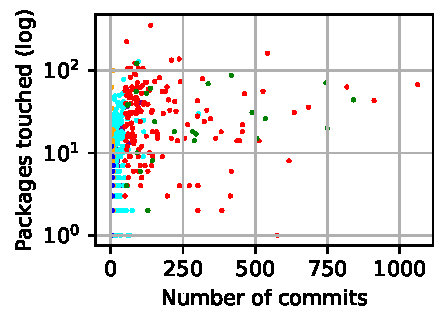
\includegraphics[width=\textwidth]{sections/results/graph/sample_scatter_touched_against_commit.packages.sample.first.pdf}
    \caption{Packages}
    \label{figure.sections/results/graph/sample_scatter_touched_against_commit.packages.sample.first.pdf}
  \end{subfigure}
  \begin{subfigure}[b]{0.45\textwidth}
    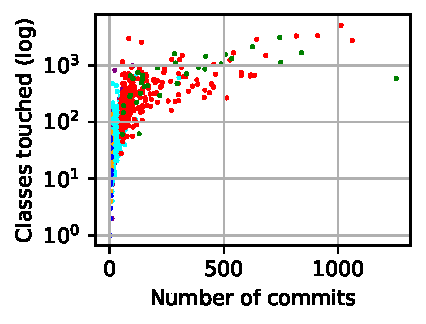
\includegraphics[width=\textwidth]{sections/results/graph/sample_scatter_touched_against_commit.classes.sample.first.pdf}
    \caption{Classes}
    \label{figure.sections/results/graph/sample_scatter_touched_against_commit.classes.sample.first.pdf}
  \end{subfigure}
\vspace{3mm}
  \begin{subfigure}[b]{0.45\textwidth}
    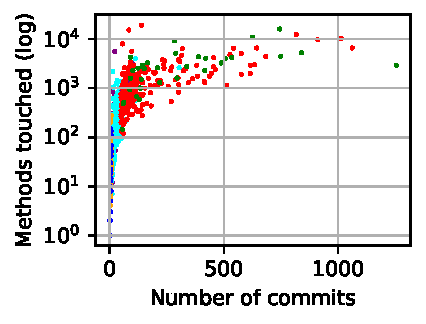
\includegraphics[width=\textwidth]{sections/results/graph/sample_scatter_touched_against_commit.methods.sample.first.pdf}
    \caption{Methods}
    \label{figure.sections/results/graph/sample_scatter_touched_against_commit.methods.sample.first.pdf}
  \end{subfigure}
\caption{Scatter plots of the log total number of components touched (y-axis) against the number of commits (x-axis) made by samples of developers capped at 203 sustained later joiners from six (6) categories: \color{Blue}Transient Founder (Blue, 203), \color{Purple}Moderate Founder (Purple, 41), \color{Green} Sustained Founder (Green, 34), \color{Orange} Transient Later Joiner (Orange, 203), \color{Cyan}Moderate Later Joiner (Cyan, 203), \color{Red} Sustained Later Joiner (Red, 203). \color{Black}} 
\end{figure}
\clearpage 
